\chapter{Experiment to Compare Various Implimentations on Real and Synthetic Data}

This chapter outlines the exact procedures that are carried out in an experiment to determine the performance capabilities of Bayesian inference for electron density profile inference within a tokamak.

The methodology goes through the values used for including prior information. It describes the algorithms used to compute the hyperparameter \gls{map} and sample for the full Bayesian method.

The results systematically provide the inferences for each method on real and synthetic data. It includes an analysis of the findings.

\section{Methodology for hyperparameter MAP and full Bayesian experiment}
The previous section outlined the procedure for using Bayesian inference to solve a simple regression problem. It then expanded the concept to inferring the electron density profile with interferometry data. This included the possibility of placing prior information into the likelihood through artificial observations. The density at the plasma boundary is artificially observed to be 0 with an artificial Gaussian error of $0.5 \cdot 10^{19}$. The profile gradient at the magnetic axis $(\rho=0)$ is artificially observed to be 0 with a Gaussian error of $0.01$. \gls{map} was introduced as a way to optimise the hyperparameters. The full Bayesian analysis method is introduced as marginalisation over the hyperparameters. The results from both methods will be presented. Both methods allow for hyperpriors to be included. A uniform prior is used for all hyperparameters and the bounds were selected by carefully observing how the parameters affect the resulting inference. The amplitude is constrained between $0$ and $100$ and is on the same scale as the electron density $10^{20}$. Each length scale is bounded between $0$ and $3$ and is on the same scale as the normalised radius. This includes the two non stationary kernel options; hyperbolic tangent length scale and cubic spline length scale. 5 knots were used for the cubic spline. To reduce the dimensionality of the problem the knots were evenly spaced across the normalised radius. Each interferometry channel is given the same experimental error bounded between $0.03$ and $0.3 \, \cdot 10^{19}m^{-2}$. \gls{west} reports a no plasma noise in the order of $0.03 \cdot10^{-19}m^2$. 

\begin{figure}[H]
    \centering
    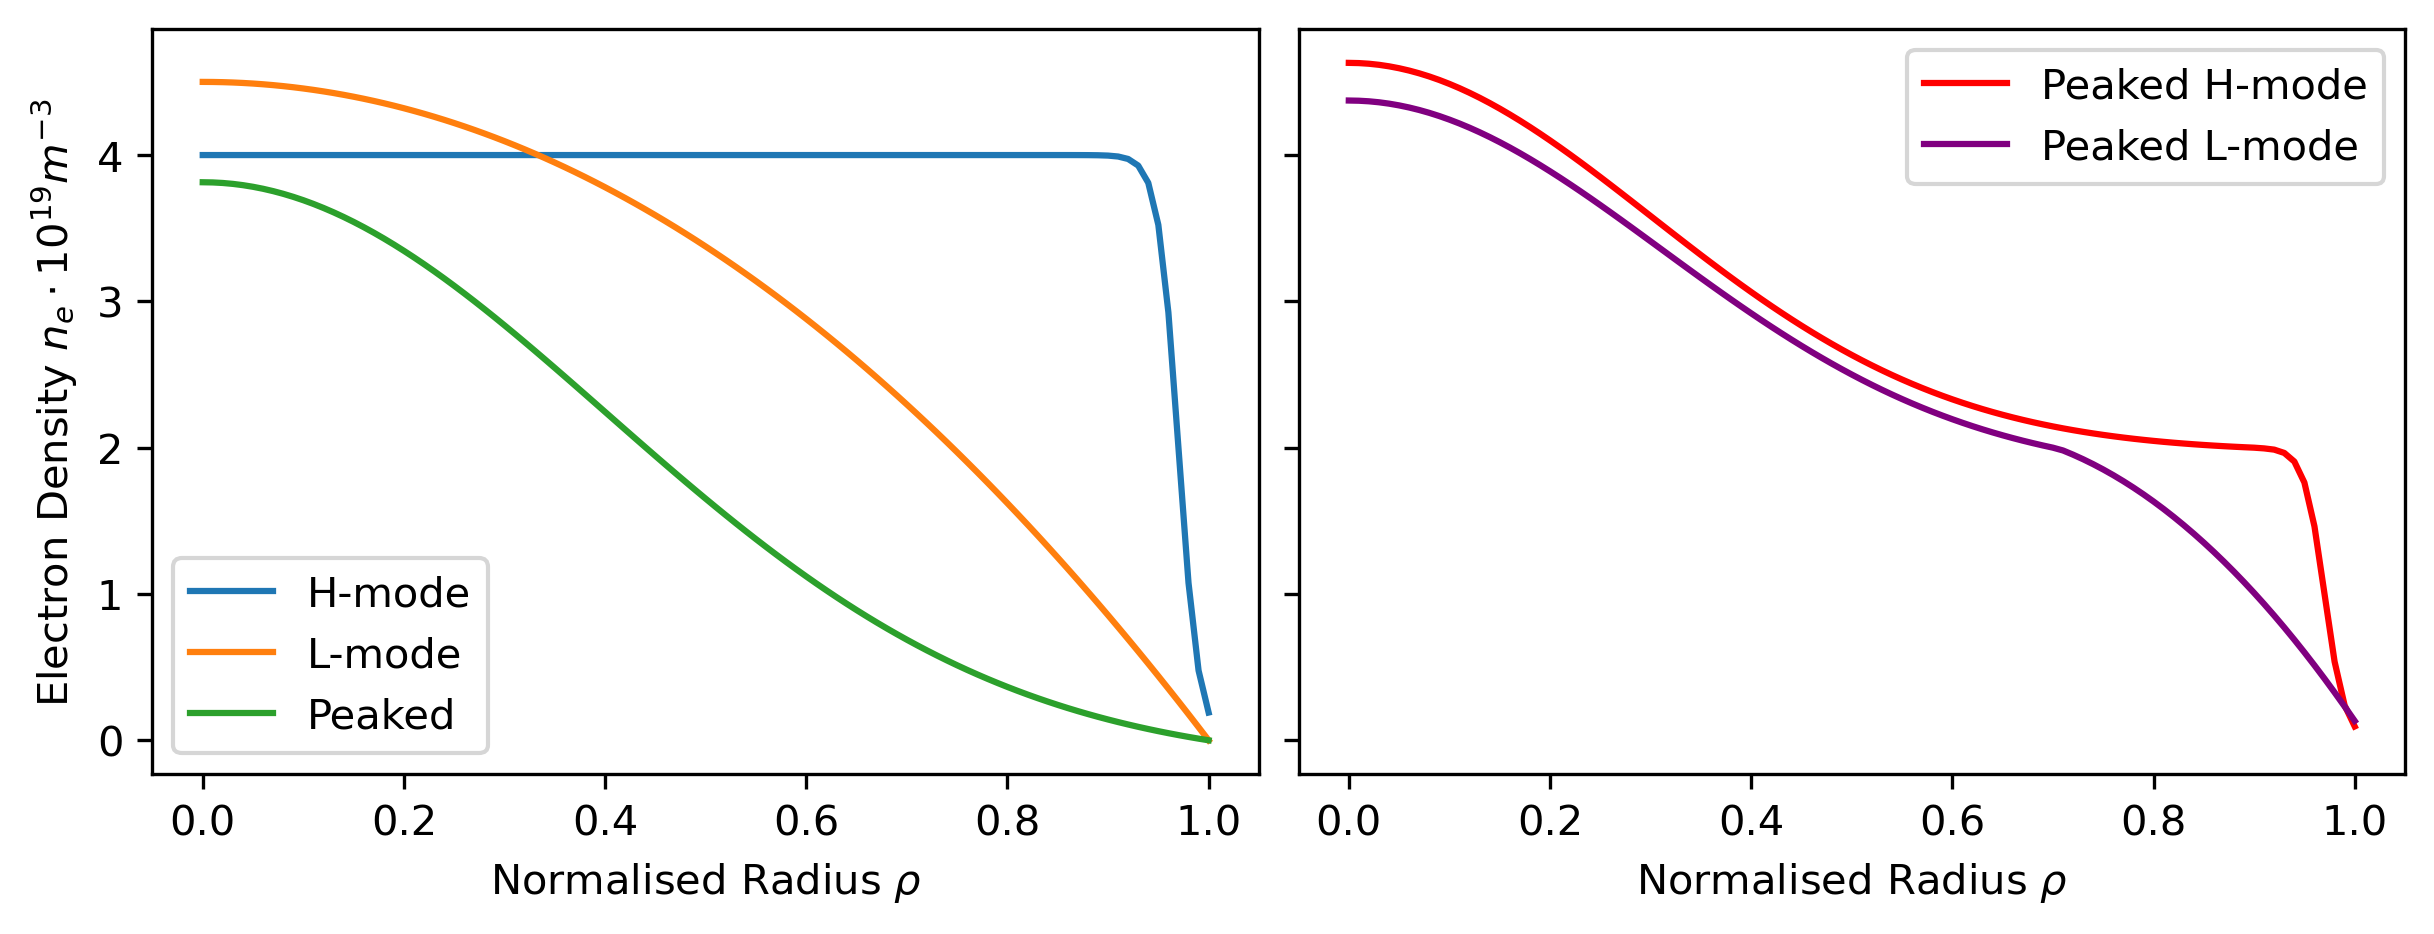
\includegraphics[width=\textwidth]{images/syntheticProfiles.png}
    \caption{Common tokamak profiles used to generate synthetic interferometry data.}
    \label{fig:groundtruth}
\end{figure}

The mean squared error between the inferred profiles and synthetically created ground truth profiles will be computed. This allows precise performance comparisons between the kernels and hyperparameter methods. There are a few main profile types of interest to the scientific community. L mode or low confinement profiles are typically parabolic like in shape. They are the bread and butter of tokamak operations. It is the easiest profile to achieve and is often a stepping stone to achieving other profiles within a plasma shot. This is the main profile used within the \gls{west} tokamak. H mode or high confinement mode is achieved by increasing external heating power from sources such as neutral beam injection and electron cyclotron resonance heating. H mode profiles have a distinct sharp drop in density near the plasma boundary. H mode profiles are well known for largely increasing the energy confinement time of the plasma which is a crucial factor for net positive energy production. Although H mode introduces extra instabilites known as ELMS. Another interesting profile feature is known as peaking. The external heating elements can be tuned to target the core. The extra heat ionises more of the fuel and decreases electron-ion recombination rates. This increases the electron density in the core and creates a peak or bell shaped profile. This can be achieved with both L mode and H mode. Peaking is known to increase the stability and performance of the plasma. It helps reduce the impurities in the core that contribute to radiation loss. The profiles are defined as shown in figure \ref{fig:groundtruth}, and converted into synthetic error free interferometry data via the response matrix. The response matrix is created using real magnetic field lines inferred by \gls{nice}. A small Gaussian experimental error is added with a standard deviation of $3\cdot10^{17} \, m^{-2}$. This is what \gls{west} reports as the no plasma noise of the interferometer.

The hyperparameter \gls{map} is found by minimising the loss function based on the marginal likelihood, see equation \ref{eq:loss}. When any trialed parameters exceed their prior bounds the loss returns infinity (or a very high number). `SciPy minimize' and `PyTorch SGD' are both gradient based methods that were trialled and achieved similar results.

The full Bayesian approach involves using \gls{mcmc} to sample from the hyperparameter posterior. This thesis uses the emcee python package which is based on the affine-invariant ensemble sampler proposed by Goodman and Weare \cite{emceeGoodman}. This method uses many `walkers' that explore the parameter space in parallel. They update their positions using the proposal function and the position of another walker. The advantage of this method is that it is invariant to affine transformations of the parameter space. Since a unique posterior distribution can be analytically computed from the hyperparameters, sampling hyperparameters is equivalent to sampling many posterior distributions. Each posterior is a multivariate Gaussian. This thesis uses the Scipy stats multivariate Gaussian random variable sampler, to sample one profile $\vec n_e$, from each posterior. Overall this is equivalent to sampling from a posterior that is independent of the hyperparameters $P(\vec n_e | \vec d)$. The mean density at each normalised radius forms the full Bayesian inferred profile. The standard deviation is computed for uncertainty. Using the mean and standard deviation allows for a direct comparison to the \gls{map} results. The distribution of $n_e$ at a point of the normalised radius is plotted to show it is Gaussian like, see figure \ref{fig:ne_dist}. The median and quantiles are also acceptable measures.

\begin{figure}[H]
    \centering
    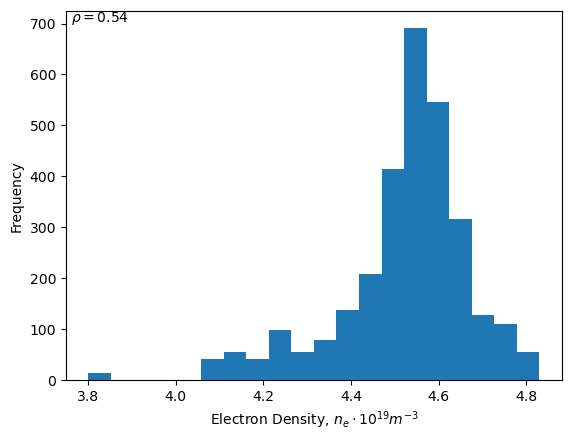
\includegraphics[width=250pt]{images/Final/sampled_ne_dist.png}
    \caption{An example distribution of $n_e$ for $\rho=0.54$ from the full Bayesian sampling method.}
    \label{fig:ne_dist}
\end{figure}

To minimise autocorrelation the emcee hyperparameters are tuned. The main hyperparameter is called `moves', which is their term for the proposal function. It is possible to pass multiple moves and weights when sampling. Emcee will randomly select a move in proportion to the weights. This should make the next sample more random and less correlated to the previous. Each move also has a single parameter. Optuna is a hyperparameter tuning framework for Python that proposes trials in an attempt to minimise the objective function. By default, it uses the tree-structured Parzen estimator algorithm. In this thesis four of the moves and their parameters are trialled with Optuna. Each trial was allowed to take 500 samples and 100 trials were made for the stationary kernel. The autocorrelation for each chain on each parameter is averaged. For each move, the trial with the lowest average autocorrelation time is found. The moves parameter value for this trial is recorded. The weights are calculated to allow the best performing move to be used more frequently, see figure \ref{fig:optuna}. 

\begin{figure}[H]
    \centering
    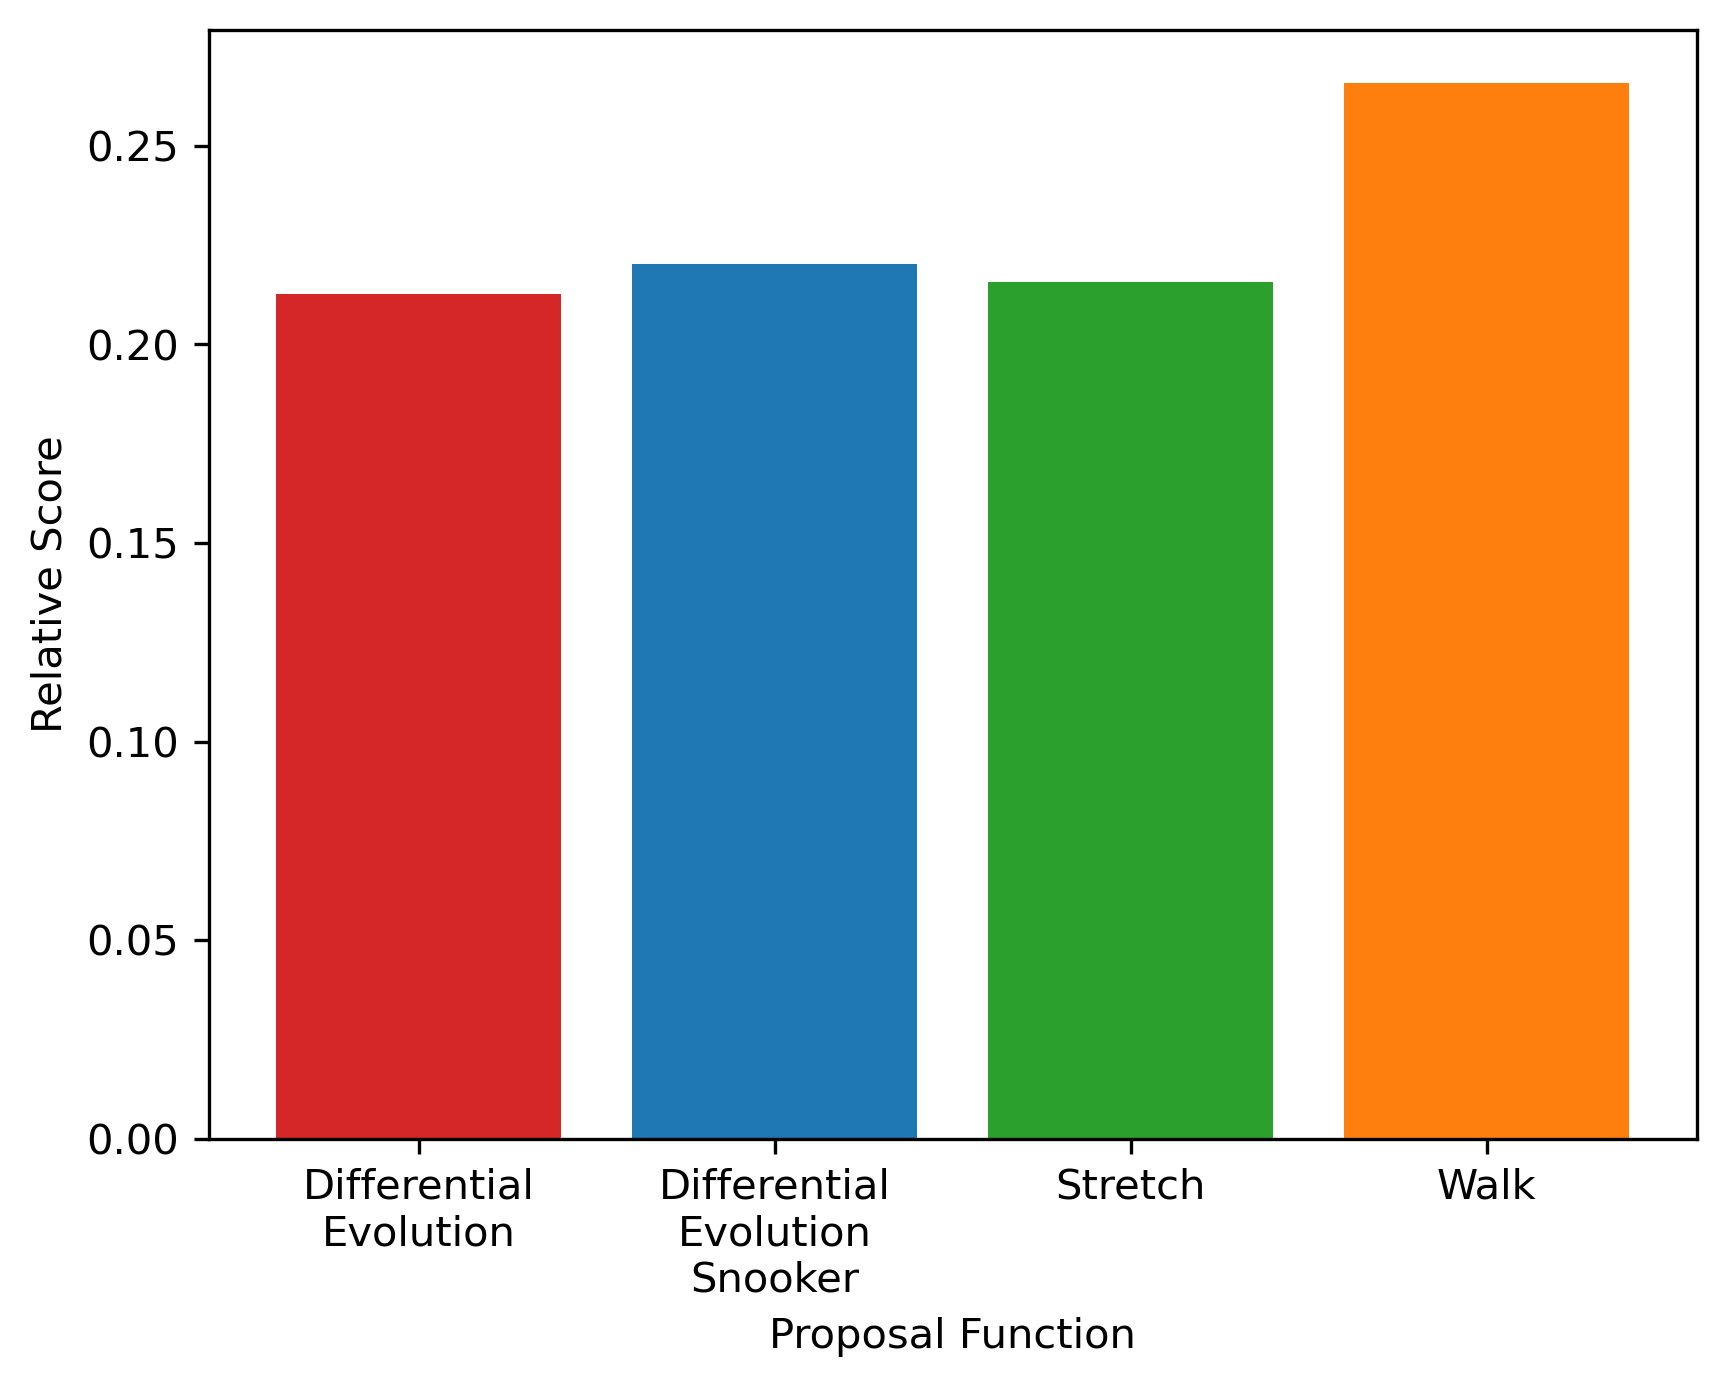
\includegraphics[width=380pt]{images/Final/optuna.png}
    \caption{The distribution from which emcee proposal functions (moves) are selected based on performance in an Optuna evaluation.}
    \label{fig:optuna}
\end{figure}

Tuning the emcee moves was not repeated for each kernel to save on computation. For each full Bayesian inference 6000 samples are collected using the tuned moves, 1000 are burned and the rest are thined by degree 10. An example chain of the remaining 500 samples has an integrated autocorrelation time of 23.6, see figure \ref{fig:tracethin}. This is still a significant amount of autocorrelation that could affect the reliability of the results.

\begin{figure}[H]
    \centering
    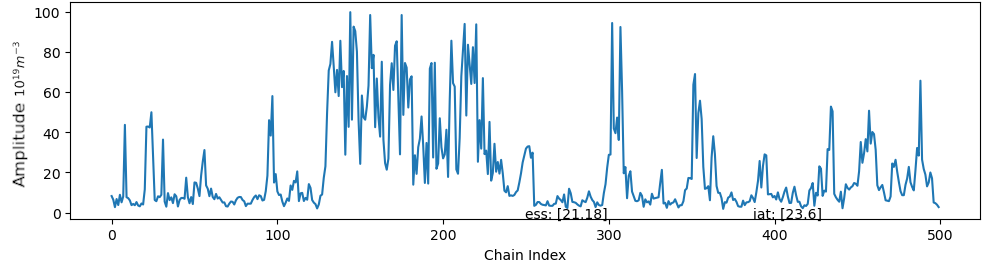
\includegraphics[width=400pt]{images/Final/TraceBurn1000_thin10.png}
    \caption{A trace plot showing the amplitude samples left after a burn of 1000 and thin of degree 10 are applied to 6000 samples collected with the tuned moves. The integrated autocorrelation time and the effective sample size are shown as `iat' and `ess', respectively.}
    \label{fig:tracethin}
\end{figure}

The same analysis is executed for real interferometry data from the \gls{west} tokamak. \gls{west} operates in L mode and figure \ref{fig:interf_nice} shows a \gls{nice} inference for a typical set of interferometry data and magnetic flux surfaces.

\begin{figure}[H]
    \centering
    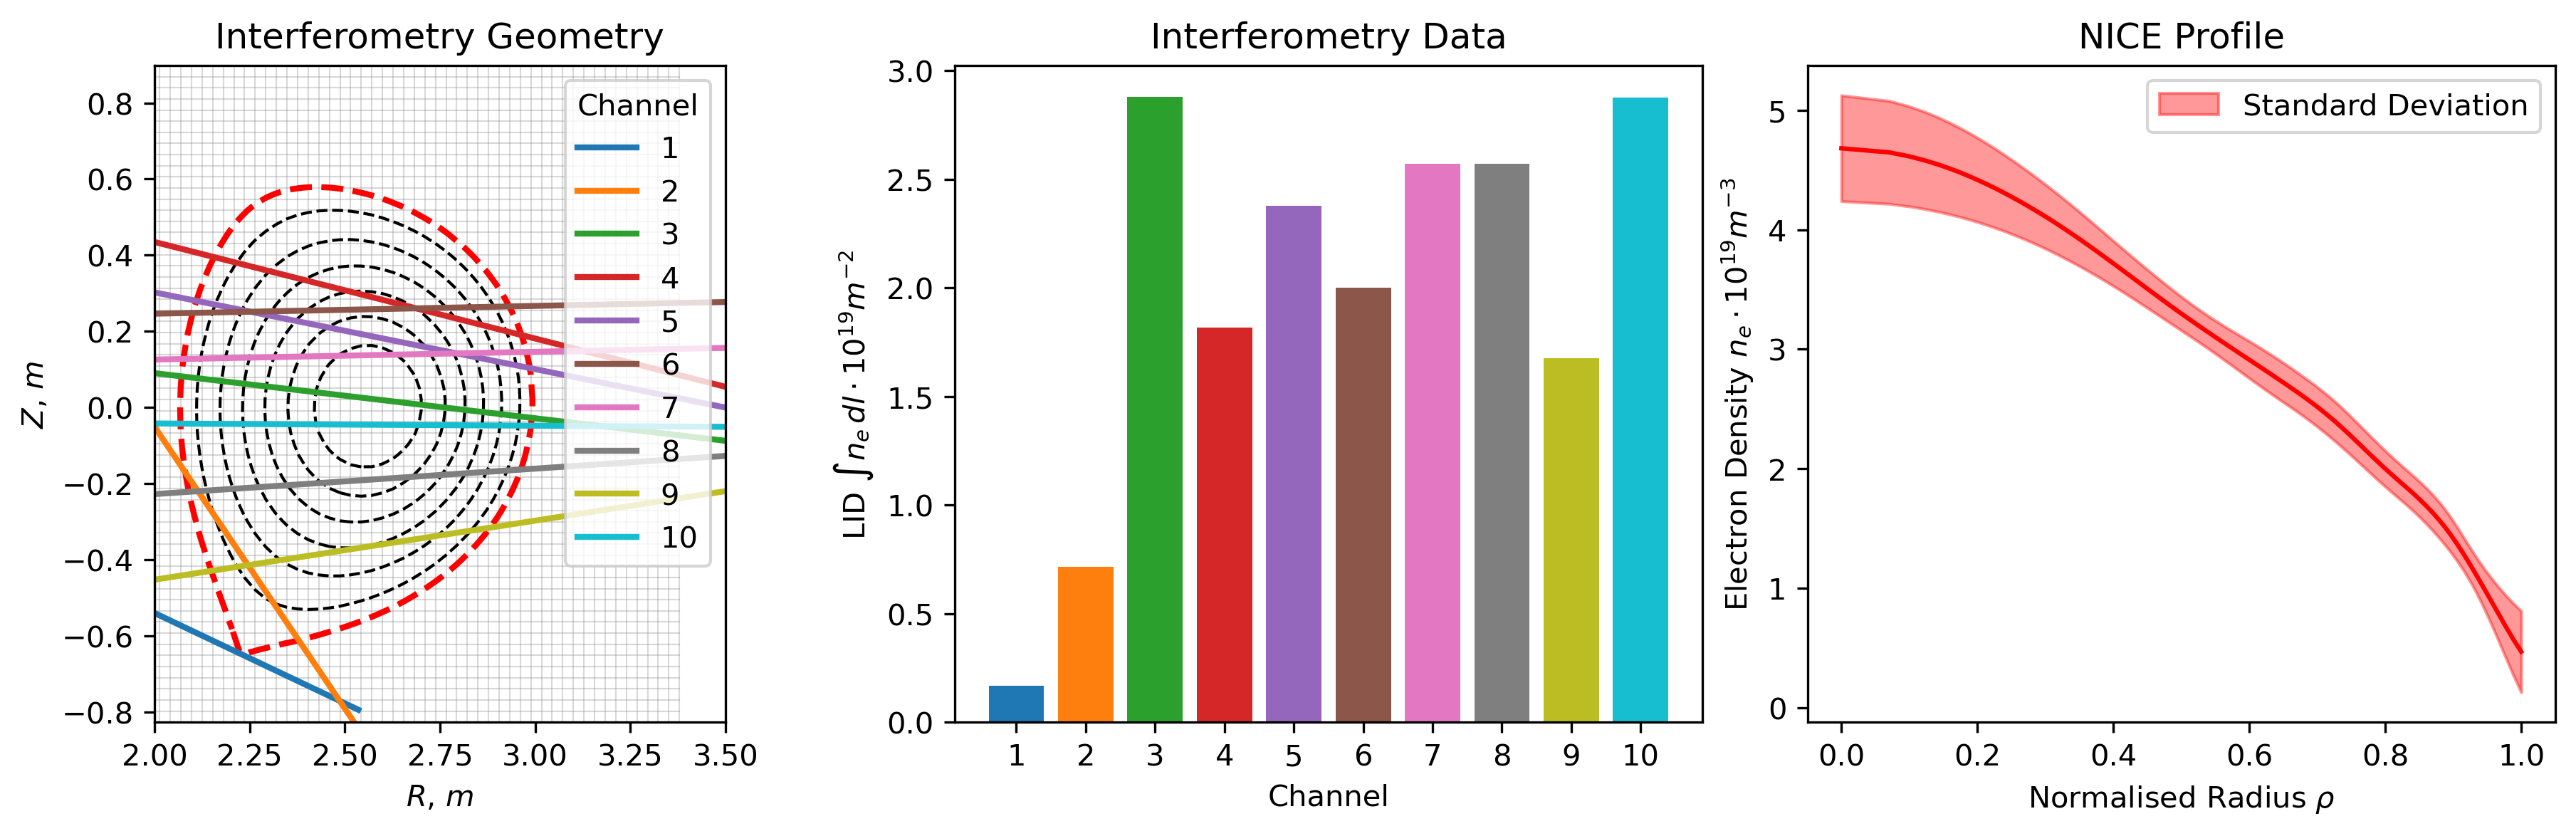
\includegraphics[width=\textwidth]{images/Final/interferometry_nice.png}
    \caption{A typical set of magnetic flux surfaces and interferometry data from the WEST tokamak. The electron density profile; inferred by the NICE algorithm.}
    \label{fig:interf_nice}
\end{figure}

As seen in the results section there are some unexpectedly poor inferences. To determine if this is due to a limitation of the kernel, a manual adjustment of the stationary kernel is performed. This is in general not a true inference as it involves knowing a reference profile to approach.

\section{Resulting Desnity Profiles of each Implimentation}

% The following inferences systematically go through the previously described kernels, methods for hyperparameter handling and data options. Their ability to match the reference profile is indicated by the mean square error between the profiles, `mse'.

As expected the hyperbolic tangent was the most successful at inferring the H mode profile, see figure \ref{fig:mapsynthetic}. This is because the constant flat top requires a high length scale yet the sharp drop requires a low length scale. A low length scale reduces the correlation between neighbouring inferred electron densities which is required for the high gradient at the edge. It is impressive how equally accurate and precise the three kernels are at inferring the L mode profile. The static kernel performed poorly when faced with a more complex shape such as the peaked L and H mode profiles. It appears close to parabolic and this is likely due to the inferred length scale being too large. The cubic spline length scale showcases its flexibility, allowing it to find some of the profile features although this appears to come at a price of smoothness. The hyperbolic tangent was able to find the H mode edge but not as closely as it was in the pure H mode profile. It still outperformed the other kernels for the H mode peak. The hyperbolic tangent has the lowest mean `mean square error' over all the profiles at $0.053$. Cubic splines are second with $0.076$ and the stationary kernel performed the worst with $0.129$, see figure \ref{fig:mapsynthetic}.

\newgeometry{top=3cm}
\begin{figure}[H]
    \centering
    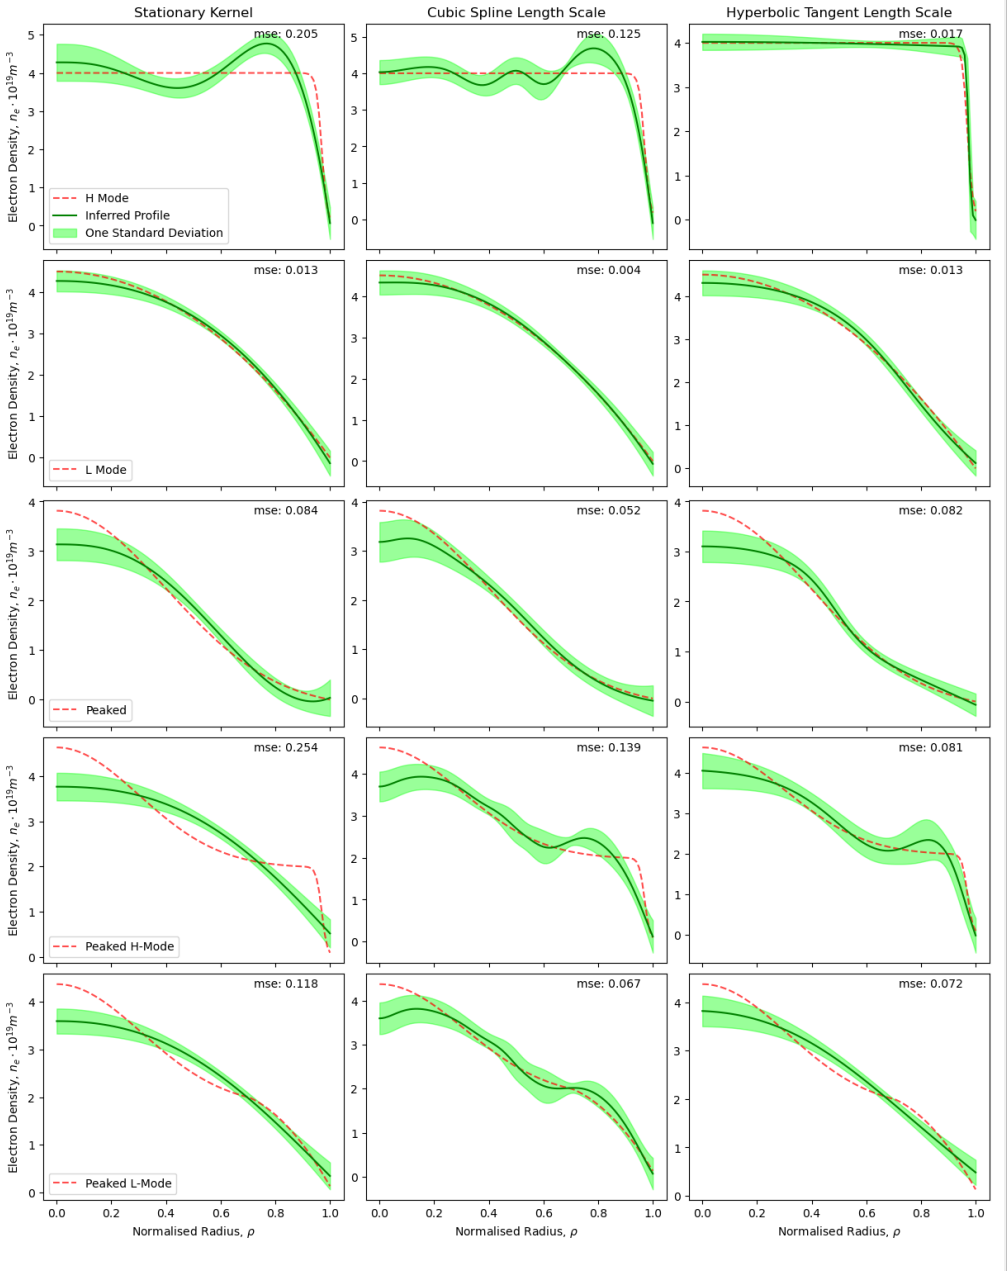
\includegraphics[width=\textwidth]{images/Final/MAPsynthetic_final_all.png}
    \caption{Electron density inference using the hyperparameter MAP method on synthetic interferometry data. The mean square error is shown as `mse'.}
    \label{fig:mapsynthetic}
\end{figure}
\restoregeometry 

For the H and L mode profiles the full Bayesian analysis performed similarly well to the hyperparameter \gls{map} method, see figure \ref{fig:fbsynthetic}. The \gls{map} method fits closer to the ground truth with an average mean squared error of $0.06$ over the L and H mode profiles, compared to $0.13$ for the full Bayesian method. Surprisingly the full Bayesian method performed poorly when faced with peaked profiles. It seems unable to follow the features of the profile and often conforms to a parabolic like shape. Both the \gls{map} and full Bayesian methods have this issue with peaked profiles but the full Bayesian amplified the problems and caused it to occur for more of the profiles. Overall the inferences from the hyperparameter \gls{map} method have an average mean squared error of $0.09$ compared to $0.19$ from the full Bayesian method.

\newgeometry{top=3cm}
\begin{figure}[H]
    \centering
    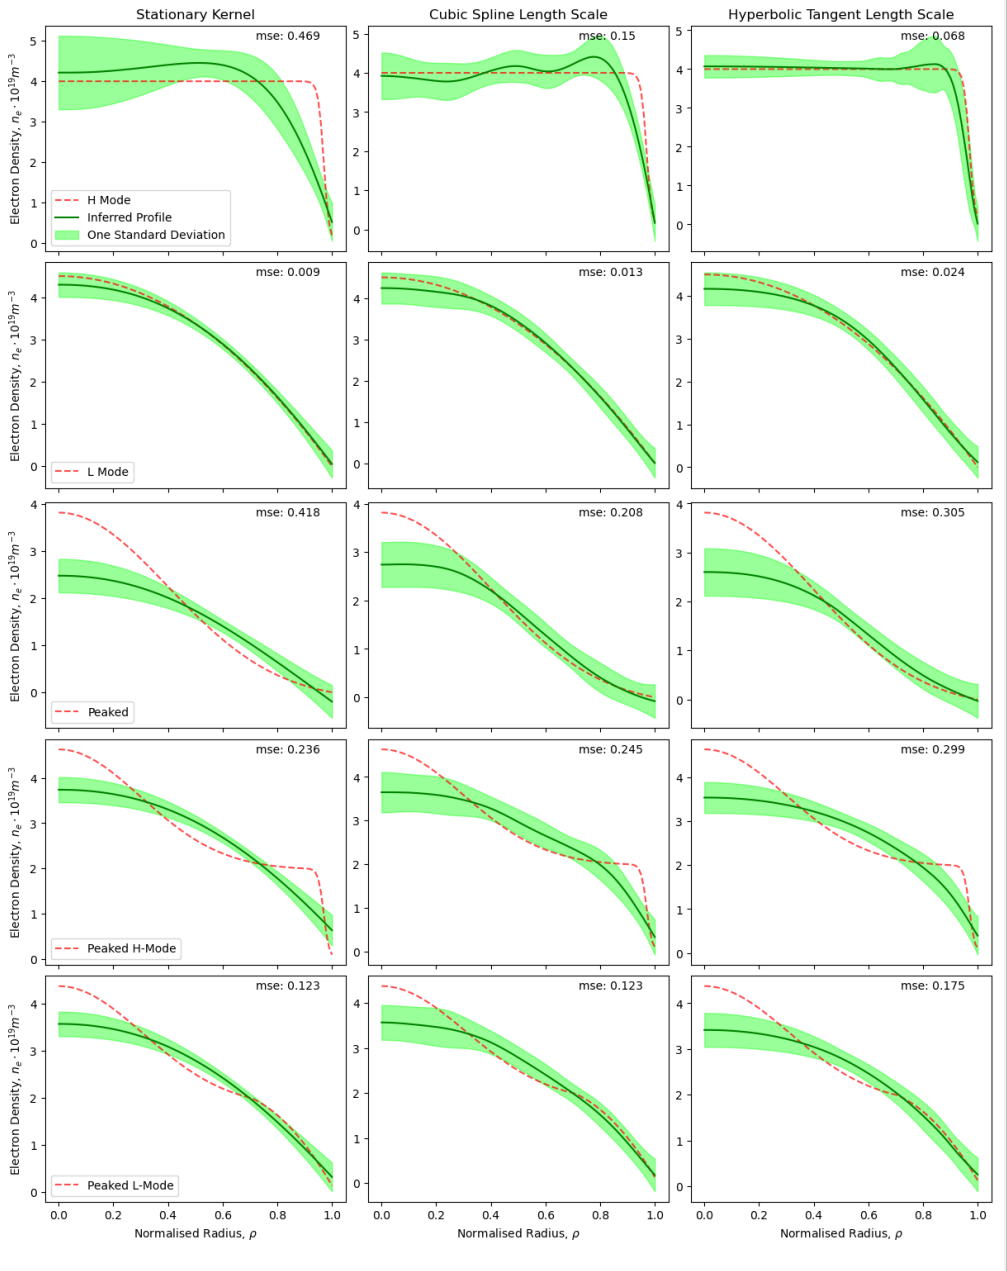
\includegraphics[width=\textwidth]{images/Final/FBsynthetic_all.png}
    \caption{Electron density inference based on the full Bayesian method for synthetic interferometry data. The mean square error is shown as `mse'.}
    \label{fig:fbsynthetic}
\end{figure}
\restoregeometry 


The same analysis is executed for real interferometry data from the \gls{west} tokamak. The inferences from the hyperparameter \gls{map} method are shown in figure \ref{fig:map_real}. The L mode profile in \gls{west} is often not close to a perfect parabola as used in the synthetic data investigation. As \gls{nice} has found, it often has an almost linear region in between the core and edge that flattens in the core and plunges to 0 near the edge. This happens with no attempts of peaking or high confinement. Despite being L mode, these extra features have caused the \gls{map} method to struggle, see figure \ref{fig:map_real}. 

\begin{figure}[H]
    \centering
    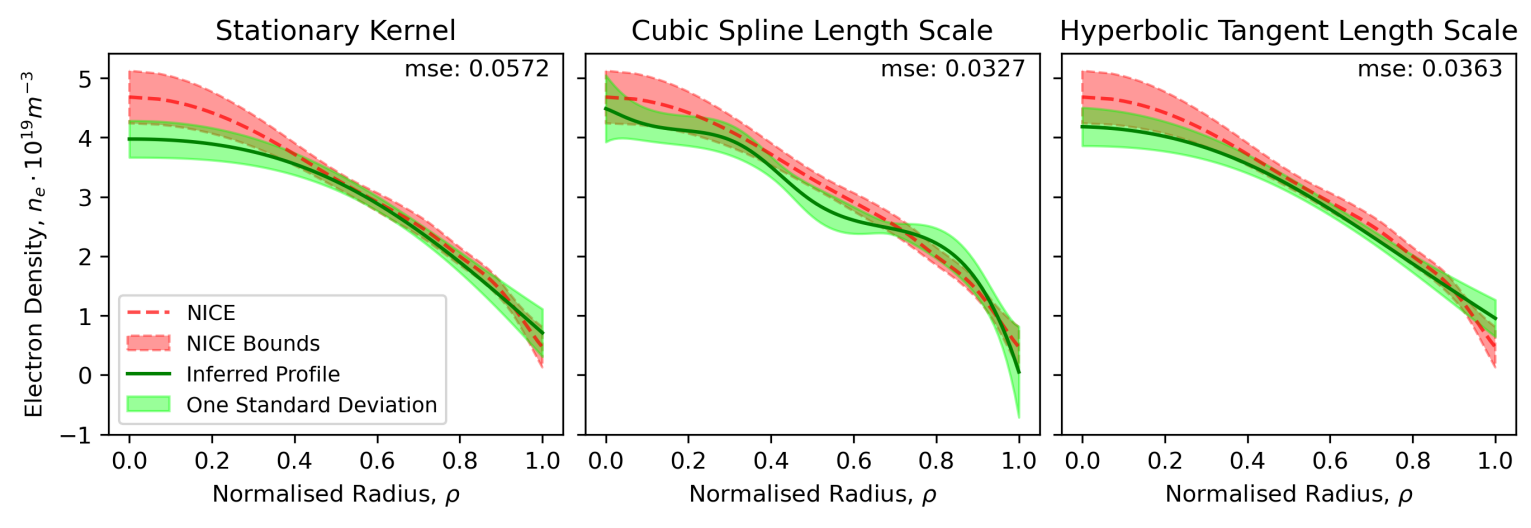
\includegraphics[width=\textwidth]{images/Final/map_real.png}
    \caption{Electron density inference using the hyperparameter MAP method on real interferometry data from the WEST tokamak. The mean square error is shown as `mse'.}
    \label{fig:map_real}
\end{figure}

By comparing figures \ref{fig:map_real} and \ref{fig:fb_real} we see that the mean square error shows that the \gls{map} method is closer to \gls{nice} for both the cubic spline and hyperbolic tangent kernel. The static kernel performed similarly in both methods. However, the full Bayesian method with the hyperbolic tangent can find the small kink feature near the edge.

\begin{figure}[H]
    \centering
    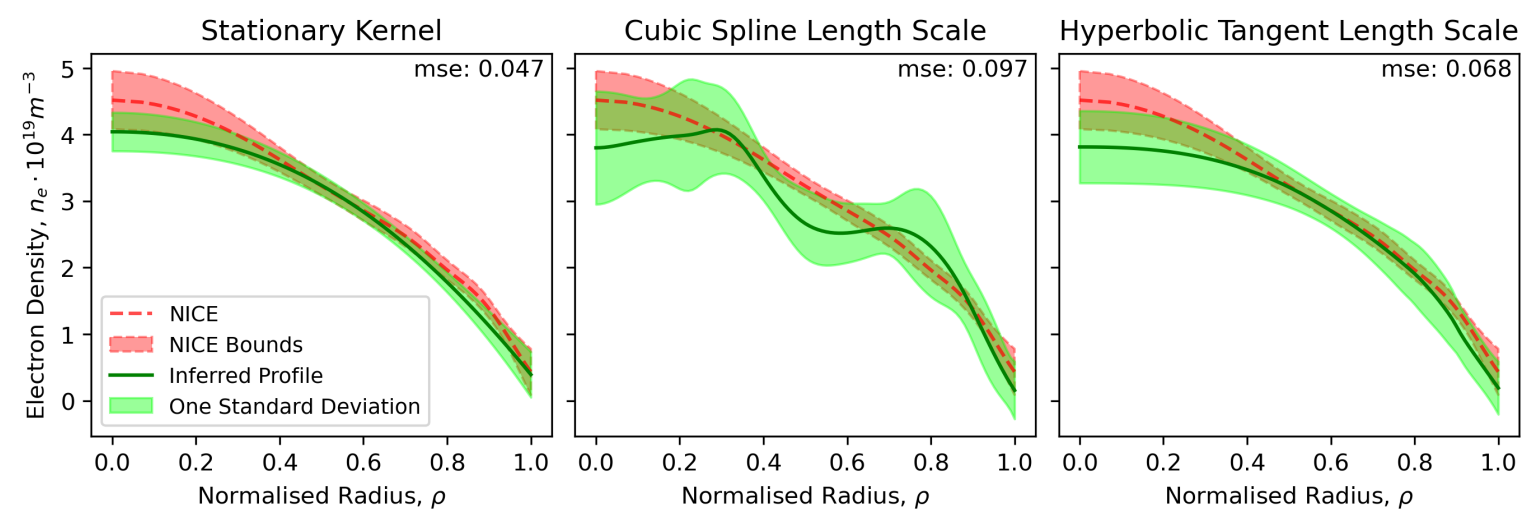
\includegraphics[width=\textwidth]{images/Final/FB_real.png}
    \caption{Electron density inference using the full Bayesian method on real interferometry data from the WEST tokamak. The mean square error is shown as `mse'.}
    \label{fig:fb_real}
\end{figure}

The final method used to optimise the inference is manual intervention. For many of the inferences with the static kernel, the length scale seems to be too large as the inferred profile appears parabolic and fails to match the shape of the ground truth or NICE. Lowering the length scale manually allows the inference to have more freedom and match more features, see figure ref{fig:manual}. This caused the mean `mean square error' of the \gls{map} method's stationary kernel to drop from $0.15$ to $0.03$ for the three inferences manually adjusted. This indicates that the hyperparameter \gls{map} method does not guarantee the most accurate possible inference. This manual intervention is in general not a true inference as it involves knowing a reference profile to approach. It was only performed to show that the kernels themselves are not at complete fault for poor results.

\begin{figure}[H]
    \centering
    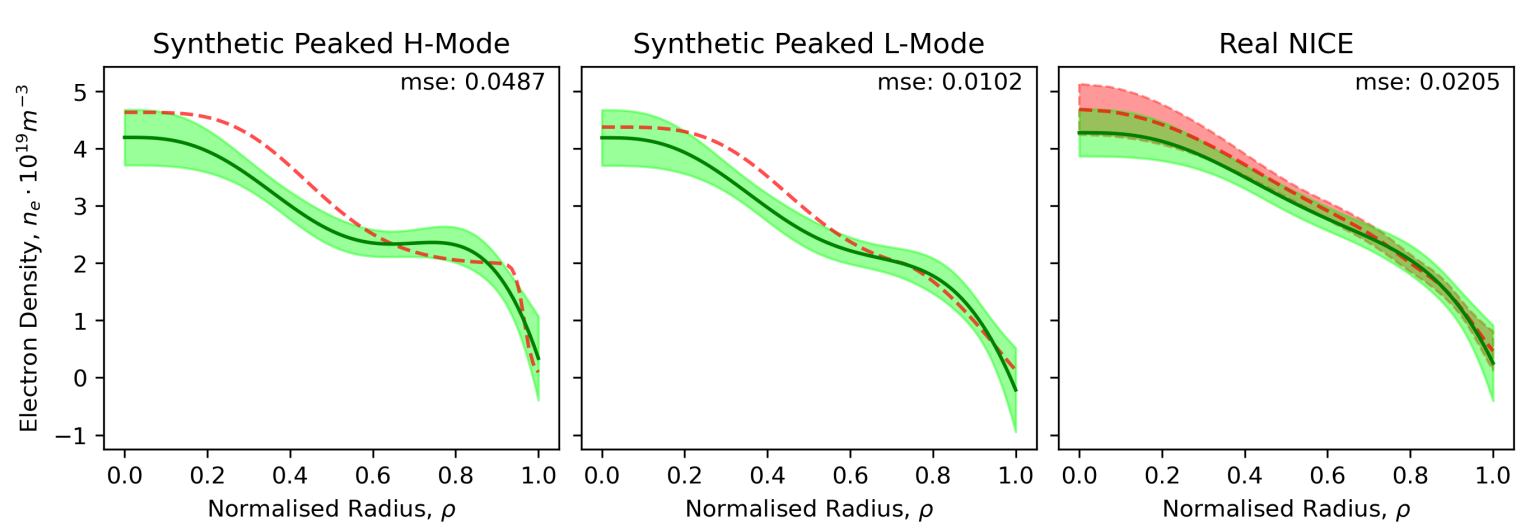
\includegraphics[width=\textwidth]{images/Final/manual.png}
    \caption{Electron density inference on real data using the stationary kernel with manually adjusted parameters. The amplitudes are set to 100, with an experimental error of 0.03 and a length scale: 0.4, 0.6 and 0.75 from left to right. The mean square error is shown as `mse'.}
    \label{fig:manual}
\end{figure}

\section{Chapter Summary}

Each hyperparameter has been given a uniform prior with specific bounds. Artificial observations were included to ensure a density near 0 at the plasma boundary and a gradient near 0 at the magnetic axis. Five profiles of scientific interest have been created and used to generate synthetic interferometry data. Real data was collected for a typical shot from the \gls{west} tokamak. An alternative inference from \gls{nice} is available for the real data. Gradient based techniques are used to determine the \gls{map} of the hyperparameters. For the full Bayesian approach the proposal function of the \gls{mcmc} sampler is tuned with Optuna. This was an attempt to reduce the autocorrelation. The autocorrelation remained unacceptably high and potentially undermines the credibility of the full Bayesian results. The results showed that profiles containing multiple features are difficult for any of the tested methods to approach. A strong H mode profile can be well inferred using a hyperbolic tangent kernel with both the \gls{map} and full Bayesian approaches. A parabolic L mode profile can be well inferred with any of the kernels and approaches. The peaked profiles contain the most features and proved the most challenging to infer. From manually adjusting the static kernel a profile was found that more closely matches the peaked profiles and the NICE profile. This shows that the kernel is not the main component holding back the quality of the results. It is more likely that the true MAP has not been found and the autocorrelation is preventing the full Bayesian samples from representing the true posterior.



% \begin{table}
% \centering
% \begin{tabular}{|c|c|c|}
%     \hline
%     \textbf{Hyperparameter} & \textbf{Lower Bound} & \textbf{Upper Bound} \\
%     \hline
%     Amplitude & 0 & 100 \\
%     Length Scale & 0 & 3 \\
%     \hline
%     \textbf{Hyperbolic Tangent} & &\\
%     Transition Center & 0 & 1 \\
%     Transition Width & 0.01 & 0.5 \\
%     \hline
%     \textbf{Cubic Spline} & & \\
%     5 Knots Evenly Spaced in $rho$ & & \\
%     \hline
% \end{tabular}
% \caption{}
% \label{tbl:prior}
% \end{table}

%methodology

% Explain the details of the how the theory is implimented, what processing power is required, I used python jupyter notebooks numpy, scipy and pytorch. Explain the key parts of the code in order to compute the kernels, marginal likelyhood and inference. What test were done in order to try and improve the inference. 

% \begin{itemize}
%     \item What format was the data in when it came from west and how did I import it into python
%     \item A bit about the diffent forms the data comes in on the west imas database and which one was chosen. 
%     \item How can the accuracy of the forward model be tested and how should this effect the experimental error.
%     \item How does one select an experimental error, is it important for the inference? 
%     \item What is the non-positive definite matrix error, how can it be avoided, what are the implications of this
%     \item How I used meshgrid to compute the kernel in a fast way
%     \item what are the different methods used for finding the minimum of the marginal likelyhood, scipy minimize, pytorch, grid search. How do they work. 
%     \item What distributions did I use to randomly initialize the kernel parameters. Why did I randomly initialise them?
%     \item Why I coded everything with pytorch tensors
%     \item How I optimised the learning rate
%     \item Attempts to use noise
%     \item How did I try and improve the inference.
%     \item summarise the chapter and lead into the results. 
    
% \end{itemize}


% \begin{itemize}
%     \item Make the case as why a 0 mean prior is not always a good Idea, since the marginal likelyhood is not perfect and inferences favour the lower side of NICE, likely due to the 0 prior as when amp is increased the inference will move to NICE but not beyond it. Including prior knowledge when available is always advised.
    
%     \item Make the case that if I set NICE as the true ground truth and create synthetic data then I get the NICE profile from lowering marginal likelyhood. This shows that everything is set up correctly.
    
%     \item Show I am getting a local minimum of the marginal likelihood which is nice like and a lower minimum which is parabolic. This could be a result of the marginal likelihood not being a perfect loss function for problems with little data. This seems to be true for SciPy, PyTorch, static and non-static.
%     \item Talk about the discovered more defined ridge, ask for access to log book to see if this is during a H-mode shot. Explain why it might be physically significant but a full monte carlo bayesian should be carried out to verify this. 
%     \item Show the static grid search

%     \item Results not yet curated
%         \subitem Bayesian inference using monte carlo methods
%         \subitem One size fits all kernel for real time. 
%     \item summarise the chapter and lead into conclusions
% \end{itemize}




%Figure \ref{fig:trace6000} shows a trace plot for the static lengthscale samples from a 6000 sample chain. 
% \begin{figure}[ht]
%     \centering
%     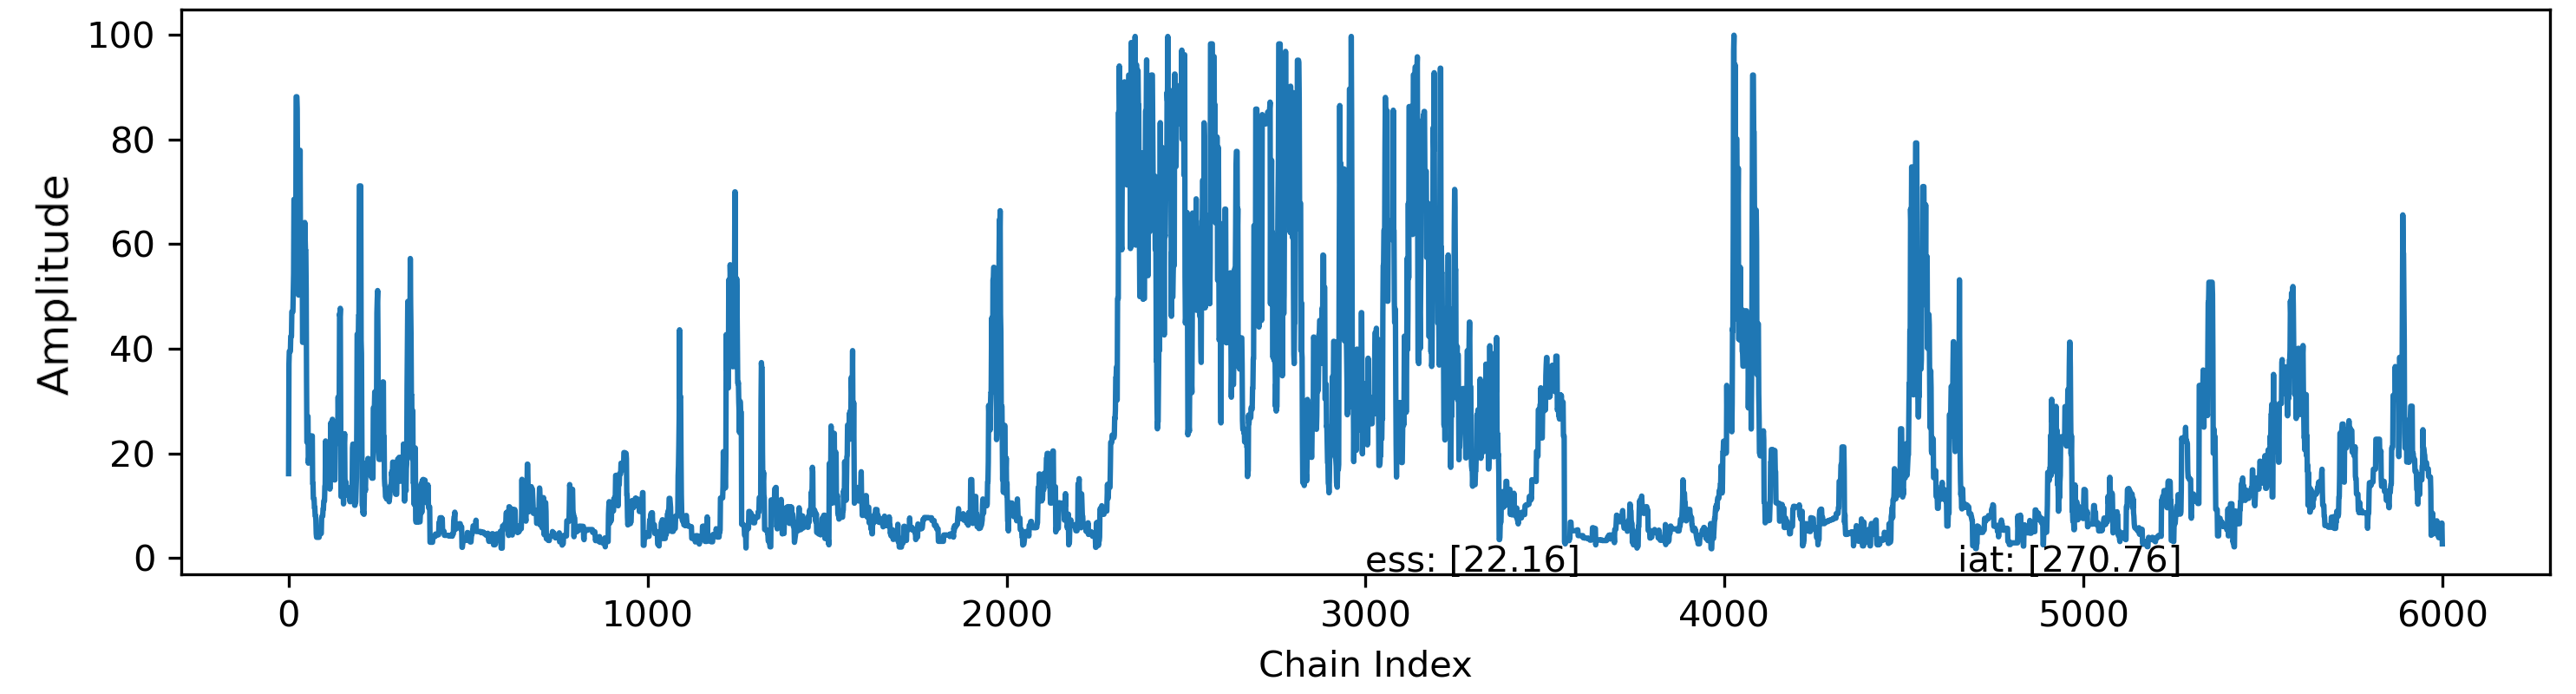
\includegraphics[width=\textwidth]{images/Final/Trace.png}
%     \caption{A trace plot showing the 6000 amplitude samples taken by an emcee chain. The integrated autocorrelation time and effective sample size is shown as `iat' and `ess', respectivly.}
%     \label{fig:trace6000}
% \end{figure}